\documentclass[twoside]{book}
\usepackage[utf8]{inputenc}
\usepackage{makeidx}
\usepackage{graphicx}
\setcounter{tocdepth}{2}
\usepackage{hyperref}
\hypersetup{pdfborder={0 0 0},colorlinks=false}
\usepackage{verbatim}
\newenvironment{smallverbatim}{\endgraf\small\verbatim}{\endverbatim}
\newenvironment{tinyverbatim}{\endgraf\scriptsize\verbatim}{\endverbatim}
\pagestyle{plain}
\usepackage{float}
\usepackage{pdfpages}
\usepackage{listings}
\usepackage[paperwidth=18.91cm,paperheight=24.59cm,top=2cm,bottom=4cm]{geometry}
\usepackage{xcolor}


\author{Federico Campoli}
\title{PostgreSQL Database Administration \\ Volume 2 \\ Architecture}
\date{First edition, 2015, some rights reserved} 

\makeindex

\lstdefinestyle{pgsql}{
  belowcaptionskip=1\baselineskip,
  breaklines=true,
  frame=l,
  language=SQL,
  showstringspaces=false,
  basicstyle=\footnotesize\ttfamily,
  keywordstyle=\bfseries\color{green!40!black},
  commentstyle=\itshape\color{purple!40!black},
  identifierstyle=\color{blue},
  stringstyle=\color{orange},
  morekeywords={VACUUM, FULL, ANALYZE, TABLESPACE,SET,ALTER, SYSTEM}
}


\begin{document}
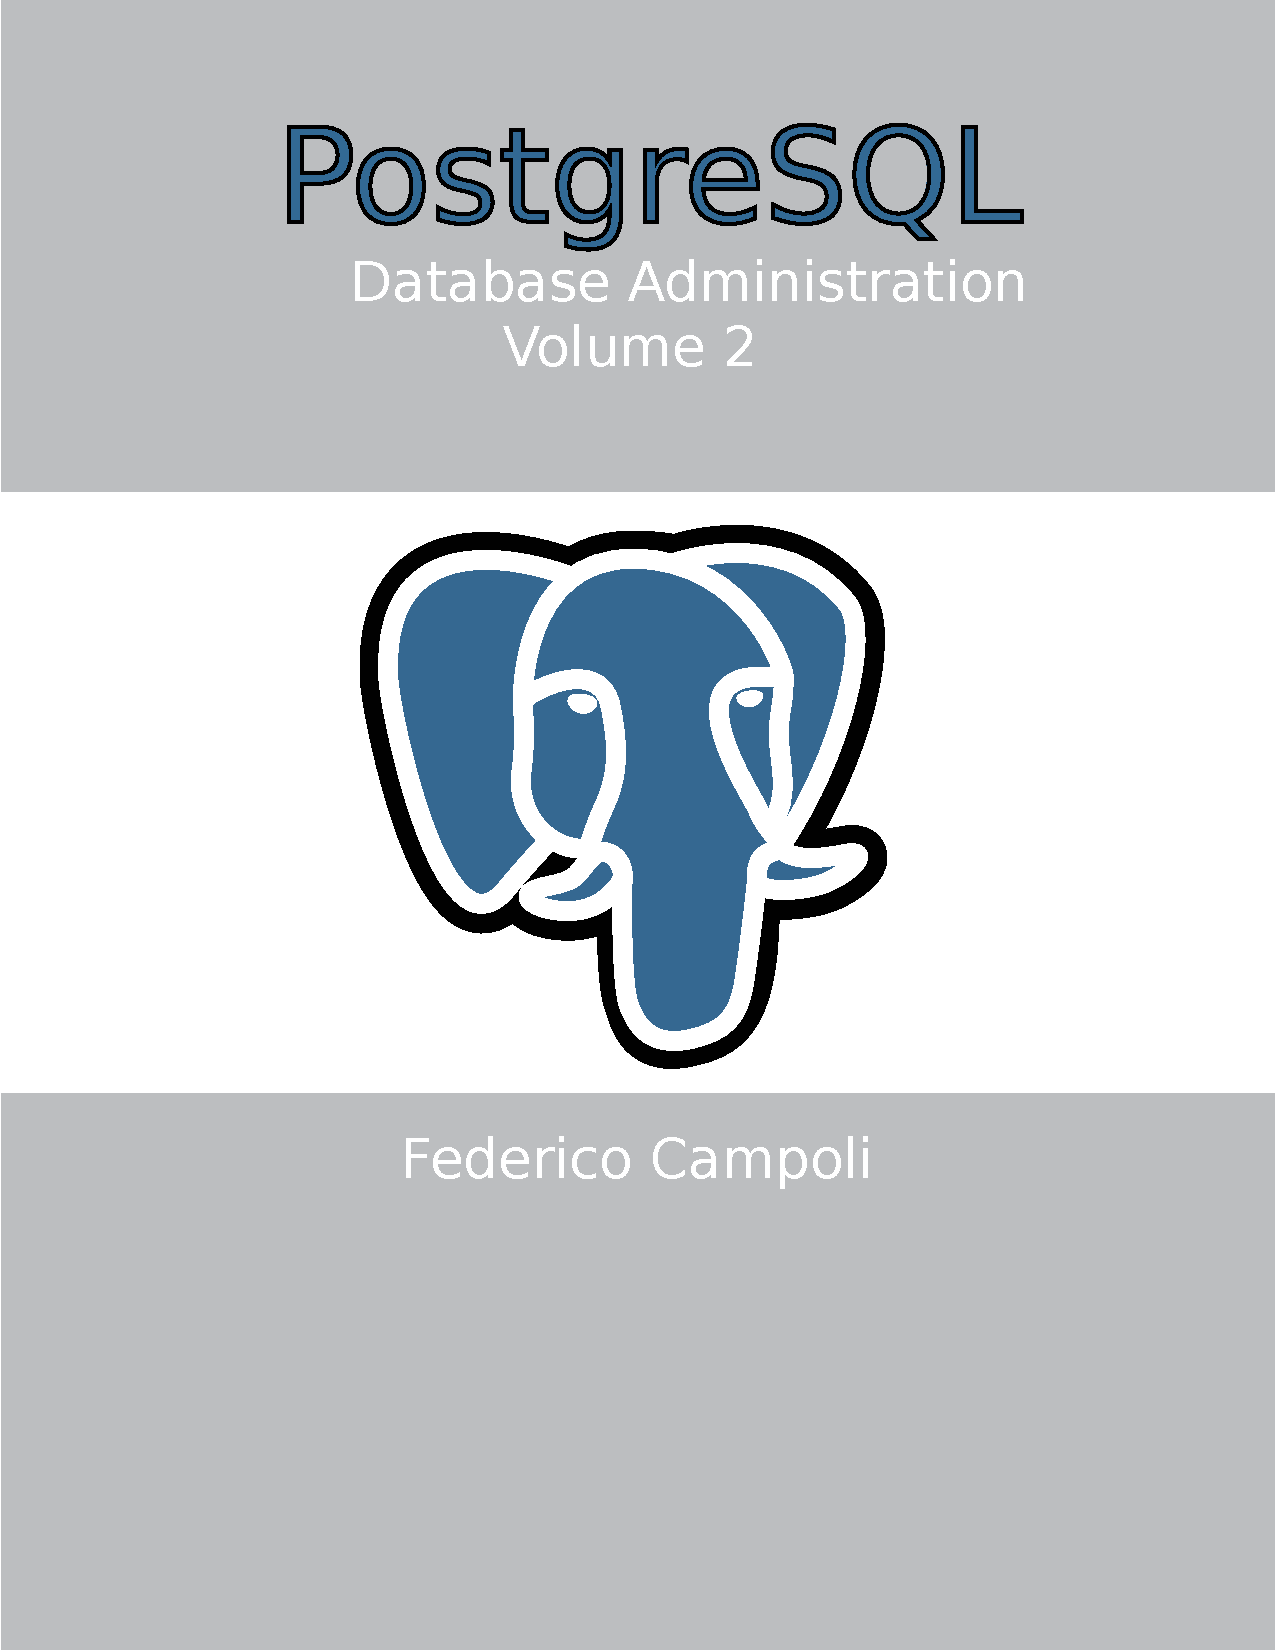
\includepdf{covers/cover_good.pdf}
\maketitle



\chapter*{License}
\begin{center}
 
\includegraphics{images/cc_logo.png}
\end{center}

The book is distributed under the terms of the Attribution-NonCommercial-ShareAlike 4.0 International 
License. To view a copy of this license, visit http://creativecommons.org/licenses/by-nc-sa/4.0/.\newline


You are free to:
\begin{itemize}
 
\item     Share — copy and redistribute the material in any medium or format
\item     Adapt — remix, transform, and build upon the material

\end{itemize}


Under the following terms:
\begin{itemize}
\item    Attribution — You must give appropriate credit, provide a link to the license, and indicate if 
changes were made. You may do so in any reasonable manner, but not in any way that suggests the licensor 
endorses you or your use.

\item    NonCommercial — You may not use the material for commercial purposes.

\item    ShareAlike — If you remix, transform, or build upon the material, you must distribute your 
contributions under the same license as the original.

\item    No additional restrictions — You may not apply legal terms or technological measures that legally 
restrict others from doing anything the license permits.

\end{itemize}

\chapter*{Copyright}
PostgreSQL Database Administration Volume 2 - Architecture\newline
Federico Campoli \copyright \space 2015 \newline
First edition\newline
%ISBN ???????????\newline



 



\chapter*{Preface}
Here we go again.


The github repository where I'm sharing the latex sources  is 
\href{https://github.com/the4thdoctor/pgdba\_books}{
https://github.com/the4thdoctor/pgdba\_books}.\newline


\section*{Intended audience}
Database administrators,  Database developers, System administrators

\section*{Book structure}
This book assumes the reader knows how to perform basic user operations such as
connecting to the database and creating tables.\newline

The book starts where the first volume ends. Reading first the volume one is warmly suggested.\newline


\chapter*{Version and platform}
This book is based on PostgreSQL version 9.4 running on Debian GNU Linux 7.
References to older versions or different platforms are explicitly specified.

\chapter*{Thanks}
The beautiful cover has been made by \href{http://www.bonland.eu/}{Chiaretta e Bon }.\newline

\tableofcontents{}

\chapter{DBA in a nutshell}
A database administrator is a strange combination of theory and practice. Because is a mix of strictness 
and loose rules is quite difficult to explain what exactly a DBA does. Working with databases requires 
passion, knowledge and a combination of empathy and pragmatism which helps to understand what 
the DBMS is thinking. With the commercial products the knowledge is commonly limited by the vendor's 
documentations and the missing parts are filled by the DBA's personal experience. Working with a free DBMS 
like PostgreSQL the source code's availability facilitates the knowledge acquisition. The PostgreSQL's 
codebase is superb poetry written in C. Just reading the comments builds an intimate relation between the 
cold binary programs and the geniuses behind the PostgreSQL Global Development Group.\newline

A day in the life of a DBA does not have fixed boundaries. The ``day'' can be just one day or spawn 
over several months, if for example if there are long procedures to run inside the well controlled 
maintenance windows. Each new day is different from the previous with a combination of various duties. 
Those are the daily tasks, the monitoring, the proactive thinking and the emergency handling. Let's see 
them in detail.

\section{Daily tasks}
Under the group of daily tasks there are all the procedures which are well consolidated on the documents 
and in the DBA mind. For example, configuring the PostgreSQL's memory parameters should be something 
immediate which does not require reading the docs. Any task in this category is successful if remains 
completely unnoticed. Is not unlikely for the production environment that the routine tasks are 
performed in antisocial hours like Sunday night or early morning in the working days.

\section{Monitoring}
A system without monitoring is an one way ticket to the disaster. Whether solution is used it should be 
something simple to configure and with a decent low rate of false positives. Having a nagging monitor is 
exactly the same like not having at all. The important alerts will pass completely unnoticed. Alongside 
with the general purpose solutions like nagios there is a new interesting PostgreSQL's dedicated called 
\href{http://opm.io/}{OPM}. Configuring a passive error detector like tail\_n\_mail is a very good idea as 
well. 

\section{Proactive thinking}
The proactive thinking is the distinctive mark between a good and DBA and a cheap professional. The 
capability of building a mental map for finding any possible issue, projected in the near future, can 
make the difference between spending the night sleeping or working frantically before the next day begins. 
Reacting to the issues is fine. Trying to prevent them is much better. This kind of tasks is strictly 
related with the monitoring. For example let's consider a master and a slave configured in continuous 
recovery. Because the slave is made copying the data files we should expect both having the same size. 
A difference in size between the master and the standby server can tell us that the filesystem have some 
issues or is not correctly configured. In this example, assuming the filesystem is XFS a bloating box is 
probably caused by the \href{
http://serverfault.com/questions/406069/why-are-my-xfs-filesystems-suddenly-consuming-more-space-and-full-of
-sparse-file}{dynamic EOF allocation} introduced in the newer XFS releases.

\section{Emergency handling}
Shit happens, deal with it. Sooner or later a disaster will strike requiring all the experience and 
efficiency of the database experts for putting back the system in production state. It doesn't matter if 
the issue is caused by an user screwing up a database table, a hardware failure or a fleet of Vogon 
spaceships ready to demolish the earth. The rule number zero when in handling an emergency is \textit{never 
guess}. Guessing without knowledge can lead to the database destruction.\newline

An example will give us a better understanding on this concept. Let's consider one of the most common 
causes of outage in the linux world, the distribution's upgrade. Usually when a linux distribution is 
upgraded, is very likely that PostgreSQL will upgrade the binaries jumping to a different major version. 
Because the data area is not compatible across the major releases will prevent the cluster's start 
after the distribution's upgrade. However the fix is quite simple installing the correct PostgreSQL's 
version.\newline.

Few years ago a desperate user stranded by a linux upgrade posted a message on a message 
board. One ``expert'' guessed that pg\_resetxlog could be be useful. Before reading further please read the 
pg\_resetxlog 
\href{http://www.postgresql.org/docs/9.3/static/app-pgresetxlog.html}{
http://www.postgresql.org/docs/9.3/static/app-pgresetxlog.html} documentation. The ``expert'' guess 
transform a simple version mismatch's issue in a serious corruption to data area.

\section{Failure is not an option}
The failure is not an option. Despite this statement is quite pretentious is also the rule number 
zero for being a decent DBA. The task failure, should this be a simple alter table or an emergency 
restore, is not acceptable. The database is the core of any application and therefore is the most important 
element of the infrastructure.\newline

In order to achieve this impossible level of service any task should be considered as single shot. 
Everything must run perfectly at the first run like not having a rollback plan. However the rollback 
procedure must be prepared and tested alongside with the main task on the test environment in order to get a 
smooth restore of the previous state if required. It's also very important to keep the checklist in mind. 
Having a checklist document is good but this does not mean that the DBA should rely only on the 
document. Remembering the checklist's steps allow the DBA to catch the exact point of any possible failure 
ensuring a rapid fix when this happens.\newline

Finally, having a plan B gives to the DBA a multiple approach for the task if something goes wrong. For 
example, when dealing with normal size databases\footnote{I consider normal sized any database under the 500 
GB} is possible to implement many strategies for the disaster recovery getting the similar time needed for 
the recovery . When the amount of data becomes important this is no longer true. For example a logical 
restore takes more time than a point in time recovery or a standby failover. In this case the plan A is the 
physical restore and, if this does not work then there is the plan B, the logical recovery.


\chapter{The cluster in action}
PostgreSQL delivers his services ensuring the ACID rules are enforced at any time. This chapter will give 
an outlook of a ``day in the life'' of a PostgreSQL's cluster. The chapter approach is purposely generic. 
At this stage is very important to understand the global picture rather the technical details. 

\section{After the startup}
When the cluster completes the startup procedure it starts accepting the connections. When a connection  
is successful then the postgres main process forks into a new backend process which is assigned to the 
client for the connection's lifetime. The fork is quite expensive and does not work very well for a 
high rate of connection's requests. The maximum number of connections is set at startup and cannot be 
changed dynamically. Whether the connection is used or not for each connection slot are consumed ~400 bytes 
of shared memory.\newline

Alongside the client's request the cluster have several processes working in the background. 

\section{The write ahead log}\index{write ahead log} 
The data pages are stored into the shared buffer either for read and write. A mechanism called pinning 
ensures that only one backend at time is accessing the requested page. If the backend modifies the page then 
this becomes dirty\index{page, dirty}. A dirty page is not yet written on its data file. However the page's 
change is first saved on the write ahead log as WAL record and the commit status for the transactions is 
stored in the directory clog or pg\_serial, depending on the transaction isolation level. The wal buffers 
ready for the flush are stored into a shared buffer's area sized by the parameter wal\_buffers.  
Inside the pg\_xlog directory there are the actual WAL files organised in fixed size segments. When a 
WAL segment is full then a a new one is created or recycled. When this happens there is a xlog switch. The 
dedicated background process WAL writer\index{WAL writer} manages the writes to the WAL. This process 
is present from PostgreSQL 8.3.

\section{The checkpoint}
The cluster, on a regular basis, executes an important activity called checkpoint. The frequency 
of this action is governed by the time and space, measured respectively in seconds and log switches between 
two checkpoints. The checkpoint scans the shared buffer and writes down to the data files all the dirty 
buffers. When the checkpoint is complete the process determines the checkpoint location and writes this 
information on the control file stored into the cluster's pg\_global tablespace. In the case of an unclean 
shutdown this value is used to determine the WAL segment from where to start the crash recovery. \newline

Before the version 8.3 the checkpoint represented a potential bottleneck because the unavoidable IO spike 
generated during the writes. That's the reason why it was introduced the concept of spread checkpoint. The 
cluster aims to a particular completion target time measured in percentage of the checkpoint timeout. The 
default values are respectively 0.5 and 5 minutes which corresponds to a target time of 2.5 minutes. From 
PostgreSQL 9.2 a dedicated checkpointer process manages the checkpoint activity.


\section{The background writer}
Before the spread checkpoints the only solution to reduce the IO spike caused by the checkpoint was to 
tweak the background writer. This was one of the new features of the revolutionary PostgreSQL 8.0. The 
writer, as the name suggests, works in the background searching for the dirty buffers to write on the data 
files. The writer works in rounds. When the process awakes scans the shared buffer and stops when has 
cleaned the amount of buffers set in bgwriter\_lru\_maxpages. The process then sleeps for the time set in 
bgwriter\_delay. 

\section{The autovacuum}
The routine vacuuming is an important task to prevent the table bloat and the dreaded XID wraparound 
failure. If enabled the autovacuum launcher take care of this taks automatically. The launcer starts one 
daemon for each relation with enough dead tuples to trigger the conditions set in 
autovacuum\_vacuum\_threshold and autovacuum\_vacuum\_scale\_factor. An autovacuum daemon is a normal 
backend and appears in the view pg\_stat\_activity. Because the XID wraparound failure is a serious issue, 
the autovacuum to prevent wraparound starts even if the autovacuum is turned off.

\section{The backends}
\label{sec:CLUBACKEND}
The PostgreSQL backend architecture is the brilliant solution for ensuring the concurrent access to the 
buffers and avoid the bottleneck of a long waiting queue. When a backend needs to access a particular tuple, 
either for read or write, the relation's pages are accessed to find the tuple matching the search criteria. 
When a buffer is accessed then the backend sets a pin onto it preventing the other backends to access the 
same page. As soon as the tuple is found and processed the pin is removed and the next backend in the queue 
will get the pin. If the tuple is modified the MVCC guarantee the other backends will see the correct 
tuple's version. The process is fine grained and very efficient. Even with an high concurrency rate on the 
same buffers is very difficult to have the backends entangled.\newline

A backend process is a fork of the main postgres process. It's very important to understand that the 
backend is not the connection but a server process assigned to the connection. Usually the backend 
terminates when the connection disconnects. However, if a client disconnects ungracefully meanwhile a query 
is running and does not signal the backend, the query will continue to run and eventually will find 
that the client is disappeared.  This is bad for many reasons. First because is consuming 
a connection slot for nothing. Also the cluster is doing something useless consuming CPU cycles and memory. 
\newline

Like everything in PostgreSQL the backend architecture is oriented to protect the data and in particular 
the volatile shared buffer. If for some reasons one of the backend process crashes then the postgres 
process terminates all the backends in order to prevent the potential shared buffer corruption. The clients 
should be able to manage this exception resetting the connection when required.\newline

\section{Wrap up}
The cluster's background activity remains most of the time unnoticed. The users and the developers can 
ignore this aspect of the PostgreSQL architecture leaving the difficult taks of understanding the 
database's heartbeat to the DBA, which should have the final word on any potential mistake in the design 
specs. The next chapters will explore the PostgreSQL's architecture in details.

\chapter{The memory}
\label{ch:PGMEMORY}
The PostgreSQL memory at first sight looks simple. If compared with the complex structures implemented in 
the other DBMS to a careless reader could seem rudimentary. However, the memory and in particular the 
shared buffers implementation is complex and sophisticated. This chapter will dig down deep into the 
PostgreSQL's memory.

\section{The shared buffer}
The shared buffer is a segment allocated at cluster's startup. Its size is determined by the GUC parameter 
shared\_buffers and the size can be changed only restarting the cluster. The shared buffer is used 
to manage the data pages as seen in \ref{sec:CLUBACKEND}, which are called buffers when loaded in memory. 
Having a shared area into the RAM have also the beneficial effect of keeping the data near the CPU for 
rapid access, keeping in memory the important things and not everything. In the era of the \textit{in 
memory databases} this could seems quite obsolete but the truth is that the resources, and the money, are 
not infinite and the memory is not cheap.

\subsection{An horrible history}
\subsection{The clock sweep}
\subsection{The wal buffers}
\subsection{Memory context}

\section{The user memory}
\subsection{Work memory}
\subsection{Maintenance work memory}
\subsection{Temporary memory}

\section{Wrap up}
\chapter{The data area}

\chapter{The cluster's architecture}
A PostgreSQL cluster is composed by a directory area initialised by init db and some processes 
accessing the data on disk and into a shared memory segment, the shared buffer. Those concepts were 
described briefly in the first volume. Now we'll see them in more details.

\section{Overview}



\chapter{Point in time recovery}
\chapter{High availability}
\chapter{Logical replication}
\chapter{SQL under the bonnet}
\chapter{Performance Tuning}

\appendix

\listoffigures
\listoftables
\printindex{}
\end{document}
